\chapter{System Architecture}
\label{ch:architecture}

%Welche Teilprobleme leiten sich aus der Zielstellung weiter ab?
%Was sind die Rahmenbedingungen für die Probleme und wie können wir diese lösen.
%Wie können wir die Probleme formalisieren? Und daraus schlussfolgern, ob sich
%existierende Lösungen ableiten lassen.
%Methodik/Vorgehen (diesmal ausführlich)
%●
%Bauen Sie auf der Methodik aus der Einführung auf.
%Ein System bauen und dann beobachten (machen Sie wohl meistens)
%Analytisch (sie prüfen ein mathematisches Gerüst/Algorithmus/ Theorem)
%Jemanden aktiv Fragen (wahrscheinlich eher in den meisten Fällen nicht)
%Übersicht bzw. Architektur
%●
%z.B. wenn Sie ein System bauen. Wie sieht Ihre Architektur aus? Was sind die Resultate des
%Entwurfs? Welche Alternativen gibt es zu Ihrem Entwurf? Warum haben Sie sich gerade für
%Ihre Lösung entschieden? Was sind deren Vor­ und Nachteile?
%Welche Prozesse unterstützt die Architektur?
%Datenquellen?
%Transformationen?
%Datenverarbeitung? ●
%Anfrage­Schnittstellen
%Oder aber: Der xxx Algorithmus
%●
%Eigenschaften des Algorithmus, Komplexität
%Wie gehen Sie vor?
%Beschreiben Sie was wann passiert
%Optional: Der yyyy Algorithmus
%●
%Eigenschaften des Algorithmus, Komplexität
%Wie gehen Sie vor?
%Beschreiben Sie was wann passiert
%Zusammenfassung (ca. 0,5 Seiten)
%●
%Was haben wir in diesem Kapitel gelernt?
%Wie passt das zur Zielstellung der Arbeit
%Wie passt das zum nächsten Kapitel?

After the context in which the solution is settled has been described in \autoref{ch:basic-concepts}, \autoref{ch:requirements}
inspected Apache Flink and Apache Kafka according available sources of data and evaluated the data based on the quality. As
a result, the functional and non-functional requirements had been defined.  According to the main goals of this thesis,
the collection of system and application data from Apache Flink and Apache Kafka and storage of collected data in a
centralized persistence system, the following sub-problems derived:

\begin{enumerate}
    \item Both source systems operate as distributed systems which consists of multiple instances of Apache
    Flink Job- and TaskManagers or Apache Kafka brokers, producers and consumers respectively. The software solution proposed
    must enable the collection of data from multiple application instances to gain an overall picture of the entire system.
    \item The process of data collection mustn't cause a negative impact on source systems. Since Apache Flink and Apache Kafka
    are both systems processing large amounts of data very fast, the utilization of system resources like cpu and memory of the
    collecting system must be kept as low as possible.
    \item As a result, the data must be transfered to the storage system with as less input/output operations and as fast
    as possible, to become available for possible data consumers immediately.
    \item The system architecture must provide a mechanism for the integration of possible data consumers which are unknown at
    the point of this thesis.
\end{enumerate}

The following chapter introduces the "Collector-Platform" as a pipeline of data collection, transport and storage with the purpose
to collect data of distributed Apache Flink and Kafka and make it available for consumers that are potentially unknown at present
as fast as possible. The components will be discussed at architectural level, whereas implementation details follow in \autoref{ch:implementation}.

\section{The "Collector-Platform"}

According to the requirements in \autoref{ch:requirements}, the "Collector-Platform" is responsible to perform the
following operations, which describe the pipeline the data in running throught on each source system. Irrespective of the source system,
the sequence remains the same for Apache Flink and Kafka or any other source system observed, it just differs in the implementation of
data collection processes:

\begin{figure}[H]
	\centering
	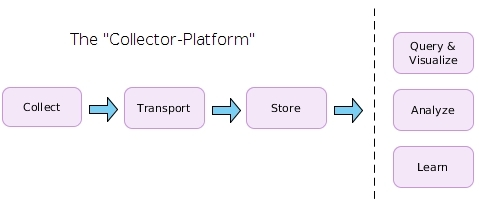
\includegraphics[width=0.8\textwidth]{../images/06-collect-pipeline.jpg}
	\caption{Collector Pipeline, \cite{VanL14}}
	\label{fig:colletor-pipeline}
\end{figure}

The the first step is the collection of data defined in \autoref{ch:requirements} on the Apache Flink and Apache Kafka source
systems. This includes collection of system data with the Dstat system utility as well as application specific data provided
by JMX or REST respectively. Once the the corresponding data had been retrieved and converted into a structured JSON format,
the data must leave source systems in the second step to reach the storage system at last, where they become available for
visualization tools, analytical processing or as a source for Machine Learning applications. \autoref{ch:evaluation} introduces
a sample application to demonstrate the possibilities for the integration of data consumers using the Stream Processing capabilities
of Apache Flink.

The "Collector-Platform" consist of the following components, that will be discussed in the following sections:

\begin{itemize}
    \item CollectorClient
%    Performs data collection based on \verb|Collector| implementations and publishes results
%    into the DataQueue, provides client metadata and an interface for scheduling the data collection process based on REST
    \item CollectorManager
    \item Consul ClientRegistry
%    \verb|CollectorClient|s register itself in this central registration, client information like host and port
%    will be available and can be queried
%    Management component, provides basic web interface for listing registered client and the scheduling of data collection
    \item Kafka Message-Broker
%     Receives the collected data from \verb|CollectorClient|s, acts as a queue for moving data across
%    the producing clients and the consumers of the data.
    \item Logstash-Processor
%     Receives and processes data from the queue, creates indexes for Elasticsearch based on the \verb|Collector|
%    implementations
    \item Elasticsearch Index
%    index that receives processed data from Logstash and stores collected in its existing JSON format
\end{itemize}

The following sections introduce the components and their corresponding functions defined above. Chosen frameworks and
technologies will not be discussed in much detail, but it will be explained why each technology or approach has been chosen.
%TODO:
%Distributed system -> distributed collection with clients,
%cloud environments, client server architecture, client-management with service-discovery, explain", communication via REST,
%Publish(client) -> Topic <- Subscribe Logstash, Data Processing Pipeline
%
%continuous, distributed, time-series "data feed", difference raw and aggregated\cite{Klepp16},
%events as "immutable facts", why? explain data samples (cpu, disk...)
%state state of system at time, on host, at port, the type of collector and data.
%
%arch uses both, raw because of unknown data consumers, flink-job-index for demonstration
%of SP.
%
%Pipeline: Collect-Transport-Persistence, see \cite{VanL14}
%
\section{The "Collector" implementations}

This set of classes builds the core for collecting data on source systems and takes the responsibility for fetching
system data (\autoref{tbl:dstatcategories}) with the Dstat system tool as well as application data for Apache Flink
and Apache Kafka using the JMX interface (\autoref{tbl:jmxjvmdata}) and via REST for Apache Flink only
(\autoref{tbl:http-api-flink}). As shown in \autoref{ch:implementation}, all implementations are based on the
\verb|Collector| interface, what enables the handling of different realizations of data collection in a uniform way.

\section{CollectorClient}

The CollectorClient is main entry point for bringing data into the platform and belongs to the "Data" layer according to
\autoref{img:taxonomy-bigdata-applications}. It is a simple Java application and will have to be installed on source systems.
The module uses the concrete \verb|Collector| implementations described above, according to the source system and
depending on which \verb|Collector|s are registered in the client. The client contains and internal registration, used for the
aggregation of an overall data result based on the data retrieved of the collectors registred.

For the scheduling purposes of the collection process, the client provides a REST resource that enables the start and stop of data
collection from the HTML user interface provided by the \verb|CollectorManager| component following in \autoref{sec:arch-collector-manager}.
This endpoint available under the location \verb|http://{client-host}:{client-port}/client/schedule| expects HTTP \verb|POST| requests
with a request body containing JSON data with an appropriate \verb|ScheduleRequest| for starting/stopping the data collection process.

Once started, the collection process that will be triggered by the client itself in a configurable interval, which is 5 seconds by default,
the resulted data will be send to an Apache Kafka topic called \verb|collector-outbound-topic|. The name of the topic explains the
purpose of the topic, it acts as the data sink for \verb|CollectorClients| and separates the clients as the producing compontent
from data consumers.

Besides the scheduling REST resource, the client contains an endpoint \newline \verb|http://{client-host}:{client-port}/client/metadata|
that provides metatdata for the individual client and is required
for displaying more detailed information about the client in the \verb|CollectorManager|.

\section{CollectorManager}
\label{sec:arch-collector-manager}
Due to the fact that Big Data Analytics Applications are composed of several interacting components and thus building
a distributed system, the "Collector-Platform" builds a distributed system itself. Based on the requirement to provide a
mechanism to schedule the collection process in distributed \verb|CollectorClient|s, the \verb|CollectorManager| represents the management
component for the distributed system of clients by providing an overview of registered clients in the platform and
the possibility to start/stop individual clients using an HTML based user interface.

\section{Consul Client-Registry}

The \verb|Client-Registry| is a dedicated web service and acts as a central registry for all data collecting components
in the platform and makes the information about registered \verb|CollectorClient|s available for the \verb|CollectorManager| instances.
For the realization of an public registry for distributed clients, the platform uses Consul, a service-registry, that enables the discovery
of web services based on unique identifiers instead of host address and port information. Since the \verb|CollectorClient| is a web service itself,
clients register itself under the service name \verb|collector-client| when the client application is started. The \verb|CollectorManager|
queries the Consul node for existing instances of services named \verb|collector-client| which results in a list of registred client instances,
that contains the required information like host and port for using the scheduling and metadata endpoints in the managers user interface.

Using an central registry instance for discovering \verb|CollectorClient| instances decouples the \verb|CollectorManager| from the
need to know detailed client information required for the localization of the service. Due to the fact that
client addresses and ports are dynamically assigned and may change in distributed cloud environments, the service registry provides
a scalable and flexible way to discover the providers of a given service.

\section{Kafka Message-Broker}

The Message-Broker integrates distributed \verb|CollectorClient|s to an overall system by providing a
message queue for transporting data from clients to the Logstash-Processor. The CollectorClients can publish
its data to the queue and the other applications can asynchronously read it from the queue at any time.

TBD
%
%Queueing, see Marz15, compute layer
%Transport, "Event-Log", see \cite{Kreps13}
%Collect the streams and make them available for consumption
%
\section{Logstash-Processor}
%
Receive messages from Message-Broker, route data, create ES index, why, describe context BDAA, compute layer
%
\section{Elasticsearch Index}

ES as search index for time-series based data, easy visualization with Kibana, why?, searchable, common in BDA, storage layer

\section{System Overview}

The following component diagram shows an overview
of all components involved and the interactions between them to fulfil the requirements of data collection, transport and storage
on the example of one Apache Flink JobManager and TaskManager as source systems:

\begin{figure}[H]
	\centering
	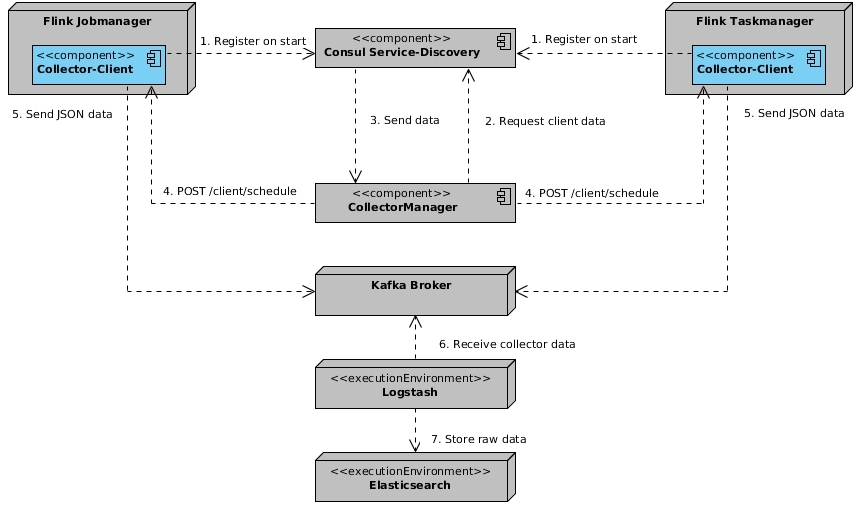
\includegraphics[width=1.0\textwidth]{../uml/component-diagram.jpg}
	\caption{The "Collector-Platform"}
	\label{fig:collector-platform}
\end{figure}

\begin{figure}[H]
	\centering
	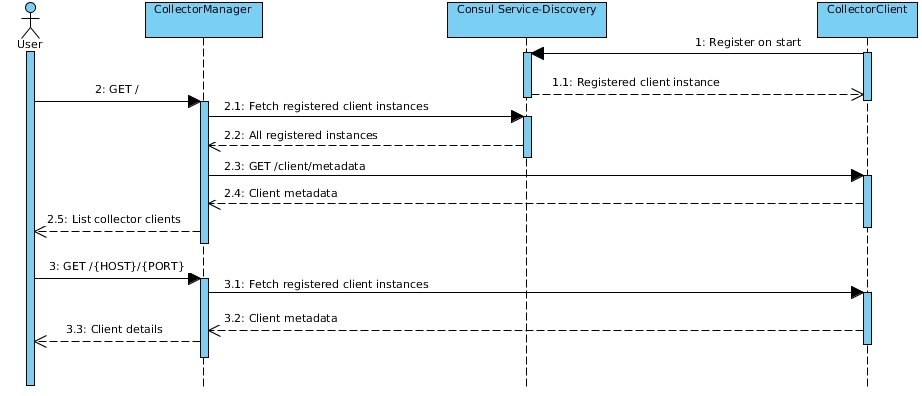
\includegraphics[width=1.0\textwidth]{../uml/sequence-discovery.jpg}
	\caption{Sequence diagram 'Client discovery'}
	\label{fig:sequence-client-discovery}
\end{figure}

\begin{figure}[H]
 	\centering
 	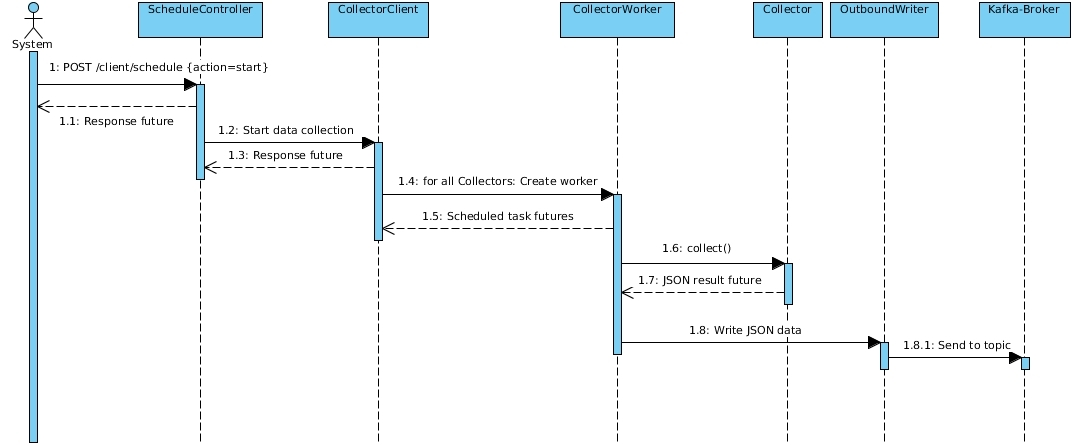
\includegraphics[width=1.0\textwidth]{../uml/sequence-scheduling.jpg}
 	\caption{Sequence diagram 'Client scheduling'}
 	\label{fig:sequence-client-scheduling}
 \end{figure}

\section{Summary}

Summarize architecture, discuss benefits and disadvantages.

software solution is a streaming platform itself,

%READ
%Messaging is the art of moving message across the producer and consumer
%group. It integrates distributed applications to an overall system by providing
%message queues for communication between them. One application can publish
%its messages to the queue and the other application can asynchronously read it
%from the queue at any time. Message Broker systems persist incoming
%messages in an enhanced type of a message queue, named topic. Sending
%messages to the broker in the form of publishing to a specific topic and on the
%other hand receiving messages only for the specified topic, is called publish /
%subscribe and this therefore classifies Kafka as a publish subscribe system.

%3.3 What is a Topic in Kafka?
%Kafka provides a high-level abstraction called Topic. Users define a new Topic
%(file) for each new category of messages (documents) and the messages are
%published to a category or stream name. A topic allows the message broker to
%deliver messages to multiple independent consumers.
%Kafka has a very simple storage layout. Each partition of a topic (file)
%corresponds to a logical log. Each time a producer publishes a message to a
%topic, the broker appends the message to the last segment file. The message is
%exposed to the consumers after it is flushed.
%
%3.4 Who are Producers in Kafka?
%Producers are the clients publishing messages to a Topic. Producers are diverse
%in nature and publish varied messages to different topics. A producer can
%publish data to a topic of its choice and is responsible for choosing which
%message will be assigned to which partition within a topic. Kafka producer client
%is configured to send messages in either a synchronous or asynchronous
%fashion to the topics. The asynchronous mode allows the client to batch small
%messages into larger data chunks before sending them over the network.
%
%3.5 What is a Message Broker?
%A Message Broker is a key element of the solution. It is a dedicated component
%which decouples the source and target systems by assuming full responsibility
%for coordinating communication between all the connected nodes. The
%published messages are stored at a set of servers called Brokers. Each Kafka
%cluster consists of one or more Brokers. The partitions of a Topic are distributed
%over the Brokers of the Kafka cluster with each Broker handling data and
%requests for a share of the partitions. Each partition is replicated across a
%configurable number of Brokers for fault tolerance. The main tasks of a message
%broker are the dynamic registration of endpoints, determining the location of a
%target system, and performing the communication as well as the transformation
%of a message from one format to another.
%A consumer can subscribe to one or more topics from the brokers and consume
%the subscribed messages by pulling data from the Brokers. The Broker locates
%the requested message by searching the list and sends the data back to the
%consumer. After a consumer receives a message it computes the location of the
%next message to consume and uses it in the next pull request.
%
%3.6 Who are Consumers in Kafka?
%The term consumer describes the clients that consume messages from a Topic.
%Producers and Consumers can simultaneously write to and read from multiple
%topics. A consumer always consumes messages from a particular partition
%sequentially. If the consumer acknowledges a particular message it implies that
%the consumer has received all the messages prior to that message. This leads to
%the fact that Kafka relies on the pull-model to reach maximum performance on
%the consumption side.
%Apache Kafka does not keep track of what messages have been consumed on
%the Broker and therefore does not rely on any acknowledgments from the
%consumer. Instead, the position of a consumer is just a single integer on a
%partition which defines the offset of the next message to consume. As a side
%benefit, it permits the consumer to rewind back to an old offset and re-consume
%data. Each consumer is represented as a process and these processes are
%organized within groups called consumer groups as Kafka supports the concept
%of consumer groups. Each consumer group consists of one or more consumers
%that jointly consume a set of subscribed topics.



